\section{Study 4 --- Technical Benchmarking}
\label{sec:method-study4}

\pgfplotsset{benchh/.style={
    xbar, /pgf/bar shift=0pt, /pgf/bar width=9pt,
    width=0.82\textwidth, height=5.4cm,
    y dir=reverse, symbolic y coords={OVH,SCW,ION,STK,TCL,AWS}, ytick={OVH,SCW,ION,STK,TCL,AWS},
    yticklabels={OVHcloud,Scaleway,IONOS,STACKIT,{T-Cloud Public},AWS},
    enlarge y limits=0.13,
    tick label style={font=\scriptsize}, label style={font=\scriptsize},
    xticklabel style={/pgf/number format/1000 sep={\,}},
    scaled x ticks=false,
    xmajorgrids=true, grid style={gray!25, dashed},
    axis lines*=left,
    nodes near coords style={font=\tiny, anchor=west, black!75},
  }}
\definecolor{bSerA}{HTML}{2563EB}
\definecolor{bSerB}{HTML}{93C5FD}
\definecolor{bNavy}{HTML}{1E3A5F}

The first three studies established whether a European provider can lawfully
protect the data it holds, whether it offers the services an enterprise needs,
and whether it has the money to keep offering them. None of them established how
well those services perform once they are running. A provider's catalogue
describes a virtual machine by its size --- two virtual processors and eight
gigabytes of memory, for instance --- but not by how quickly it computes, reads
from its disk or moves data across the network. Gillam et al.\ identified the
same gap more than a decade ago: providers state how much storage comes with a
machine, but not how fast that storage is \cite{Gillam_FairBenchmarking_2013}.
Two machines sold under the same description can therefore deliver quite
different amounts of work for the same hourly price.

This study measures that difference directly. It answers the question set for it
in \cref{tab:study-overview}: whether European providers are fast enough, and at
a price worth paying. Gillam et al.\ framed the same question as one of value for
money --- whether the cloud user gets what they pay for, or pays for what they
get \cite{Gillam_FairBenchmarking_2013}. Their Fair Benchmarking project, which
assessed Amazon, Rackspace, IBM and a private OpenStack installation with one
common set of tests, supplied the method followed here: a small number of
established benchmarks, each addressing one component of the machine, run
without any tuning for the test and compared against the best result achieved
for that benchmark \cite{Gillam_FairBenchmarking_2013}.


\subsection{Previous research on cloud benchmarking}

Benchmarking public clouds has been studied continuously since commercial
clouds first appeared, and the findings have changed as the clouds have
\cite{LeitnerCito_Chaos_2016}. The earliest studies found cloud machines both
slower and less predictable than dedicated hardware. Iosup et al.\ evaluated four
commercial cloud services, Amazon EC2 among them, and concluded that they would
need an order-of-magnitude improvement in performance to be useful for
scientific computing \cite{Iosup_ManyTasks_2011}. Schad et al.\ measured EC2 for
a month and found that its performance often fell into two distinct bands, which
corresponded to different underlying system types behind the same offer; the
variance was high enough that timing experiments on it could be run only with
considerable care \cite{Schad_Runtime_2010}.

Later work found the variation reduced but not removed, and different from one
provider to the next. Leitner and Cito reviewed the existing literature,
formulated fifteen hypotheses from it and tested them on Amazon EC2, Google
Compute Engine, Microsoft Azure and IBM Softlayer. They found substantial
differences between providers, less hardware heterogeneity than earlier studies
had reported, and a strong effect of other customers' workloads on performance,
but only at some providers \cite{LeitnerCito_Chaos_2016}. They also observed that
cloud benchmarking aims at a moving target, since providers change their
hardware and software over time \cite{LeitnerCito_Chaos_2016}. Scheuner and
Leitner then found remarkably low variability on EC2 and showed that
micro-benchmarks --- small tests of one component each, of the kind used in this
study --- could estimate the running time of a scientific application to within
10 per cent and the response time of a web application to within 10 to 20 per
cent \cite{ScheunerLeitner_MicroBench_2018}. Micro-benchmarks therefore offer a
sound basis for comparing providers when a customer's own applications cannot be
run on every one of them.

The literature has also settled what a sound cloud benchmark should report.
Bermbach et al.\ treat cloud benchmarking from the client's side: the quality of
a service is what a customer measures when using it
\cite{Bermbach_CloudServiceBenchmarking_2017}. Papadopoulos et al.\ proposed
eight principles for reproducible performance evaluation in the cloud: repeating
experiments, covering the relevant workloads and configurations, describing the
experimental set-up, making the artefacts available, describing results as
distributions rather than single values, evaluating them statistically, stating
units, and reporting cost. Their review of studies published between 2012 and
2017 found that more than two-thirds had performed no repeated experiments or
long runs, and only 21 per cent had done both \cite{Papadopoulos_Principles_2021}.
This study follows those principles where its resources allowed: every test is
repeated and reported with its lowest and highest value, the set-up and units are
stated, and cost is part of the comparison. Where it falls short of them is set
out in \cref{sec:bench-findings}.


\subsection{Existing sources of benchmark data}

Measuring six providers directly takes time and money, so the first step was to
establish whether suitable results had already been published. Gillam et al.\
surveyed the websites available when they began their work and found none of
them adequate for a fair comparison \cite{Gillam_FairBenchmarking_2013}.
CloudHarmony, which monitored some thirty-eight cloud services, sold access to
its results by the token and displayed one benchmark at a time; many of its
figures were the average of at most two measurements, and some were more than a
year old. CloudSleuth displayed response times and availability on a world map
but reported no benchmarks at all. OpenBenchmarking.org published results from
the Phoronix Test Suite for several providers, including Amazon and Rackspace,
but recorded neither the base image nor the region in which a test had been run,
so the test could not be repeated \cite{Gillam_FairBenchmarking_2013}.
CloudHarmony was reportedly absorbed into Gartner in 2015
\cite{Fortune_CloudHarmony_2015}.

Comparable sources exist today, and four were examined for the six machines in
this study:

\begin{enumerate}
  \item \textbf{Cloud Mercato} publishes measurements per provider and instance
  type in its Public Cloud Reference. It covers four of the six providers. For
  \acs{AWS}, Scaleway and T-Cloud Public it publishes network bandwidth for exactly
  the instance types tested here \cite{CloudMercato_AWS_m6i,CloudMercato_Scaleway_POP2,CloudMercato_TSystems_s3}.
  For OVHcloud and IONOS it publishes other instance sizes but not those used in
  this study, and STACKIT is not covered.

  \item \textbf{Nexxwave} published a comparison in January 2024 using the same five
  Phoronix Test Suite profiles adopted in this study, and included OVHcloud and
  Scaleway \cite{Nexxwave_2024}. It tested machines with two processors and four
  gigabytes of memory, and with four processors and eight or sixteen gigabytes,
  rather than the two-processor, eight-gigabyte size used here, and it presented
  its results only as chart images.

  \item \textbf{VPSBenchmarks} ranks virtual private server plans from a large
  number of providers, among them OVHcloud, IONOS, Scaleway and \acs{AWS}
  \cite{VPSBenchmarks_2024}. Its subjects are hosting plans grouped by monthly
  price rather than the cloud instance types assessed here, and it does not
  include STACKIT or T-Cloud Public.

  \item \textbf{OpenBenchmarking.org} still hosts the Phoronix Test Suite profiles
  and the results its users upload \cite{OpenBenchmarking_org}. No uploaded result
  was found for any of the six instance types used in this study.
\end{enumerate}

The search therefore produced one usable set of results: Cloud Mercato's network
measurements for \acs{AWS}, Scaleway and T-Cloud Public, which are used in this
study. Everything else had to be measured. Assembling partial results from
several sources would have reproduced the difficulty Gillam et al.\ describe, of
combining tests run separately with different settings, some stated and some not,
into a comparison that cannot be relied upon \cite{Gillam_FairBenchmarking_2013}.
The remaining measurements that could not be found elsewhere, were therefore measured on 10 August 2026,
by spinning up multiple machines provisioned at each provider, with the same operating
system and the same tests run throughout.


\subsection{Test environment}

Every provider was tested at the same size: two virtual processors and eight
gigabytes of memory. This is the smallest size that all six providers sell as a
machine whose full speed is included in its advertised price. Some providers
also sell cheaper machines that guarantee only a basic speed and charge extra
when they are kept busy for long periods; the \acs{AWS} T3 family works this way
\cite{AWS_T3}. The tests in this study keep a machine fully busy for their whole
duration, so on such a machine the price paid would not be the price advertised.
Each provider's standard machine was therefore used instead. Every machine ran
the same operating system, Ubuntu 22.04 LTS. \Cref{tab:bench-instances} lists the six machines, ordered by the
composite score established in \cref{sec:bench-composite}.

\begin{table}[htbp]
  \centering
  \caption{The six machines tested and where they ran, ordered by composite score.}
  \label{tab:bench-instances}
  \scriptsize
  \setlength{\tabcolsep}{3pt}
  \begin{tabularx}{\textwidth}{@{}r l >{\raggedright\arraybackslash}p{1.9cm} l c c >{\raggedright\arraybackslash}X r r@{}}
    \toprule
    \# & Provider & Instance & Location (region) & vCPU & RAM & Storage & Per hour & Comp. \\
    \midrule
    1 & AWS & \texttt{m6i.large} & Frankfurt, DE (eu-central-1) & 2 & 8\,GB & EBS gp3 (100 GB) & \texteuro0.106 & 88.4 \\[2pt]
    2 & OVHcloud & \texttt{b3-8} & Gravelines, FR (GRA) & 2 & 8\,GB & 50 GB local NVMe & \texteuro0.060 & 87.4 \\[2pt]
    3 & STACKIT & \texttt{g1a.2d} & Heilbronn, DE (EU01) & 2 & 8\,GB & Block storage (NVMe-class) & \texteuro0.098 & 82.8 \\[2pt]
    4 & IONOS & \texttt{2 vCPU /\allowbreak  8 GB flexible} & Frankfurt, DE (DE1) & 2 & 8\,GB & 100 GB SSD Premium & \texteuro0.041 & 78.0 \\[2pt]
    5 & T-Cloud Public & \texttt{s3.large.4} & Magdeburg and Biere, DE (EU-DE) & 2 & 8\,GB & EVS block storage & \texteuro0.114 & 76.0 \\[2pt]
    6 & Scaleway & \texttt{POP2-2C-8G} & Paris, FR (PAR) & 2 & 8\,GB & SBS block storage (NVMe) & \texteuro0.074 & 74.6 \\[2pt]
    \bottomrule
  \end{tabularx}
\end{table}

One difference between the machines is a property of the products rather than
of the test. OVHcloud's b3-8 keeps its data on an NVMe drive inside the same
physical server as the virtual machine, so every read and write travels over the
server's internal bus. The other five use network block storage: the disk sits on
a separate storage cluster and is reached over the provider's internal network,
which adds a delay to every operation but allows the data to be replicated. The
effect is clearest in the disk results of \cref{sec:bench-disk}, and it is
reported as measured.


\subsection{Benchmark selection}

Following Gillam et al., the tests were chosen to address the components of a
cloud machine one at a time: memory, processor, disk, a working application and
the network \cite{Gillam_FairBenchmarking_2013}. Each is introduced below by the
limitation it exposes and then by the tool used to measure it. Five of the tests
come from the Phoronix Test Suite, an open-source platform that installs and runs
standard benchmarks in a uniform way on any Linux machine
\cite{PhoronixTestSuite}; the other three measure the network and the time a
machine takes to become usable.

\begin{enumerate}
  \item \textbf{Memory (\texttt{pts/stream}).} The rate at which a processor can exchange data with memory
  limits many workloads regardless of the processor's speed, yet no provider
  publishes it. STREAM measures the bandwidth that can be sustained, rather than a
  theoretical peak, using four operations on arrays larger than the processor's
  cache: COPY moves data unchanged, SCALE multiplies it by a constant, ADD combines
  two arrays, and TRIAD combines a multiplication with an addition
  \cite{McCalpin_STREAM,Gillam_FairBenchmarking_2013}. TRIAD is the most demanding
  of the four and the closest to real workloads, and it is the one carried into the
  overall comparison.

  \item \textbf{Processor, single core (\texttt{pts/hint}).} Much real work --- serving one request,
  running a script, working through a chain of dependent calculations --- runs on
  one core at a time, and additional cores do nothing to speed it up. HINT
  (Hierarchical INTegration) isolates the speed of a single core by computing
  progressively finer estimates of an integral and counting the operations it
  completes per second, reported here in millions.

  \item \textbf{Processor, multiple cores (\texttt{pts/compress-7zip}).} A server handling many tasks at once uses
  all its cores together, and the question is whether they deliver their combined
  capacity or compete for shared resources. The 7-Zip benchmark compresses and
  decompresses data on every core simultaneously and reports the millions of
  instructions completed per second (MIPS). The compression figure is carried into
  the overall comparison.

  \item \textbf{Disk (\texttt{pts/postmark}).} Databases, mail servers and any application that handles many
  small files depend on the speed of storage, which providers describe by capacity
  rather than by rate \cite{Gillam_FairBenchmarking_2013}. PostMark creates a pool
  of small files and performs a mixture of reads, writes, appends and deletions on
  them, reporting the transactions completed per second.

  \item \textbf{Application (\texttt{pts/apache}).} A web server under load draws on the processor, the
  operating system's networking and its management of processes at the same time.
  The Apache benchmark starts an Apache web server on the machine and uses Apache
  Bench to send it requests from many simultaneous clients, reporting the number of
  requests served per second \cite{ApacheBench}. The result indicates how many
  users a machine of this size could serve before its responses begin to slow.

  \item \textbf{Network (\texttt{iperf3}).} Any application built from more than one machine depends on
  how quickly those machines can exchange data. iperf3 measures this by running as
  a server on one machine and as a client on a second machine in the same zone,
  sending data across the private network and recording the throughput in each
  direction \cite{iperf3_ESnet,Gillam_FairBenchmarking_2013}.

  \item \textbf{Provisioning (boot and set-up time).} Gillam et al.\ describe the use of a cloud machine as a
  sequence --- request, boot, set-up, run and release --- in which charging
  typically begins as soon as the request is received
  \cite{Gillam_FairBenchmarking_2013}. The time spent booting and setting up is
  therefore paid for while producing no work. Boot time is measured from the
  request to create the machine until it first accepts a secure-shell (SSH)
  connection. Set-up time is measured from that point until cloud-init, the
  component that configures a Linux machine on its first start, has finished
  initialising the operating system \cite{CloudInit}.
\end{enumerate}

\Cref{tab:bench-profiles} summarises the eight measurements.

\begin{table}[htbp]
  \centering
  \caption{The eight measurements, grouped by the categories of Gillam et al.}
  \label{tab:bench-profiles}
  \footnotesize
  \setlength{\tabcolsep}{4pt}
  \begin{tabularx}{\textwidth}{@{}l l X l c@{}}
    \toprule
    Category & Test & What it measures & Unit & Better \\
    \midrule
    Memory         & \texttt{pts/stream} (TRIAD) & Sustainable memory bandwidth         & MB/s          & higher \\
    CPU, single    & \texttt{pts/hint}           & Speed of one core                    & million MIPS  & higher \\
    CPU, multiple  & \texttt{pts/compress-7zip}  & All cores working together           & MIPS          & higher \\
    Disk           & \texttt{pts/postmark}       & Small-file transactions              & per second    & higher \\
    Application    & \texttt{pts/apache}         & Web requests served                  & per second    & higher \\
    Network        & \texttt{iperf3}             & Bandwidth between two machines       & Mbit/s        & higher \\
    Provisioning   & Boot time                   & Request until SSH is available        & seconds       & lower  \\
    Provisioning   & Set-up time                 & SSH until cloud-init has finished    & seconds       & lower  \\
    \bottomrule
  \end{tabularx}
\end{table}


\subsection{Results by component}

The results are presented in the order of the tests. Each figure shows the
average of the runs for each provider. The lowest and highest value and the
number of runs behind every average are given in \cref{tab:bench-heatmap}.

\subsubsection{Memory bandwidth}
\label{sec:bench-memory}

\begin{figure}[htbp]
  \centering
  \begin{tikzpicture}
    \begin{groupplot}[benchh,
      group style={group size=2 by 2, horizontal sep=0.6cm, vertical sep=1.35cm},
      width=0.5\textwidth, height=5cm, xmin=0, xmax=36000,
      xtick={0,10000,20000,30000}, xticklabels={0,10k,20k,30k},
      title style={font=\scriptsize\bfseries, yshift=-4pt},
      nodes near coords={\pgfmathprintnumber[fixed, precision=0, 1000 sep={\,}]{\pgfplotspointmeta}},
      nodes near coords style={font=\tiny, anchor=west, black!75},
      point meta=x]
    \nextgroupplot[title={COPY}]
      \addplot[fill=cProvB, draw=cProvB!70!black] coordinates {(30313.0,OVH)};
      \addplot[fill=cProvA, draw=cProvA!70!black] coordinates {(28583.6,SCW)};
      \addplot[fill=cProvD, draw=cProvD!70!black] coordinates {(23987.0,ION)};
      \addplot[fill=cProvE, draw=cProvE!70!black] coordinates {(27983.7,STK)};
      \addplot[fill=cProvC, draw=cProvC!70!black] coordinates {(29983.8,TCL)};
      \addplot[fill=cBase, draw=cBase!70!black] coordinates {(25247.0,AWS)};
    \nextgroupplot[title={SCALE}, yticklabels={}]
      \addplot[fill=cProvB, draw=cProvB!70!black] coordinates {(14674.7,OVH)};
      \addplot[fill=cProvA, draw=cProvA!70!black] coordinates {(16903.7,SCW)};
      \addplot[fill=cProvD, draw=cProvD!70!black] coordinates {(18346.9,ION)};
      \addplot[fill=cProvE, draw=cProvE!70!black] coordinates {(16546.9,STK)};
      \addplot[fill=cProvC, draw=cProvC!70!black] coordinates {(17646.9,TCL)};
      \addplot[fill=cBase, draw=cBase!70!black] coordinates {(19233.8,AWS)};
    \nextgroupplot[title={ADD}]
      \addplot[fill=cProvB, draw=cProvB!70!black] coordinates {(16809.3,OVH)};
      \addplot[fill=cProvA, draw=cProvA!70!black] coordinates {(19237.1,SCW)};
      \addplot[fill=cProvD, draw=cProvD!70!black] coordinates {(20243.7,ION)};
      \addplot[fill=cProvE, draw=cProvE!70!black] coordinates {(18843.7,STK)};
      \addplot[fill=cProvC, draw=cProvC!70!black] coordinates {(19960.4,TCL)};
      \addplot[fill=cBase, draw=cBase!70!black] coordinates {(21343.7,AWS)};
    \nextgroupplot[title={TRIAD}, yticklabels={}]
      \addplot[fill=cProvB, draw=cProvB!70!black] coordinates {(16944.3,OVH)};
      \addplot[fill=cProvA, draw=cProvA!70!black] coordinates {(19383.8,SCW)};
      \addplot[fill=cProvD, draw=cProvD!70!black] coordinates {(20393.7,ION)};
      \addplot[fill=cProvE, draw=cProvE!70!black] coordinates {(18993.7,STK)};
      \addplot[fill=cProvC, draw=cProvC!70!black] coordinates {(20100.4,TCL)};
      \addplot[fill=cBase, draw=cBase!70!black] coordinates {(21477.1,AWS)};
    \end{groupplot}
  \end{tikzpicture}
  \caption{Memory bandwidth, \texttt{pts/stream}, in MB/s.}
  \label{fig:bench-stream}
\end{figure}

The four operations do not place the providers in the same order.
\Cref{fig:bench-stream} shows OVHcloud with the highest bandwidth of the six on
COPY, at 30\,313 MB/s, and the lowest on each of the other three operations. On
TRIAD, the operation closest to real workloads, \acs{AWS} leads at 21\,477 MB/s,
followed by IONOS, T-Cloud Public, Scaleway and STACKIT, with OVHcloud last at
16\,944 MB/s --- a difference of 27 per cent between first and last. OVHcloud's memory
therefore moves data quickly when nothing is computed along the way, but slows
more than the others once arithmetic is added, which is the pattern most real
programs follow.

\subsubsection{Processor performance}

\begin{figure}[htbp]
  \centering
  \begin{tikzpicture}
    \begin{axis}[benchh, xmin=0, xmax=520, xlabel={million MIPS},nodes near coords={\pgfmathprintnumber[fixed, precision=1, fixed zerofill]{\pgfplotspointmeta}},point meta=x]
      \addplot[fill=cProvB, draw=cProvB!70!black] coordinates {(445.27,OVH)};
      \addplot[fill=cProvA, draw=cProvA!70!black] coordinates {(437.52,SCW)};
      \addplot[fill=cProvD, draw=cProvD!70!black] coordinates {(415.62,ION)};
      \addplot[fill=cProvE, draw=cProvE!70!black] coordinates {(424.26,STK)};
      \addplot[fill=cProvC, draw=cProvC!70!black] coordinates {(418.50,TCL)};
      \addplot[fill=cBase, draw=cBase!70!black] coordinates {(443.59,AWS)};
    \end{axis}
  \end{tikzpicture}
  \caption{Processor speed on a single core, \texttt{pts/hint}, in millions of MIPS.}
  \label{fig:bench-hint}
\end{figure}

\begin{figure}[htbp]
  \centering
  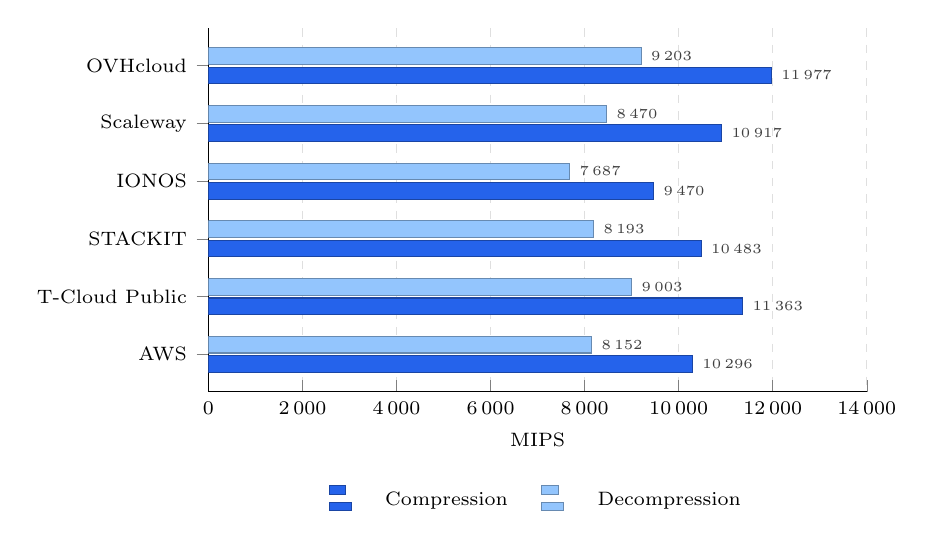
\begin{tikzpicture}
    \begin{axis}[benchh, xbar, /pgf/bar shift=0pt, height=6.2cm, xmin=0, xmax=14000,
      xlabel={MIPS},
      /pgf/bar width=6pt,
      legend style={font=\scriptsize, at={(0.5,-0.24)}, anchor=north,
                    legend columns=2, draw=none, column sep=1em},
      nodes near coords={\pgfmathprintnumber[fixed, precision=0, 1000 sep={\,}]{\pgfplotspointmeta}},
      point meta=x]
      \addplot[fill=bSerA, draw=bSerA!70!black, /pgf/bar shift=-3.5pt] coordinates {(11976.67,OVH) (10916.70,SCW) (9470.00,ION) (10483.30,STK) (11363.33,TCL) (10296.00,AWS)};
      \addplot[fill=bSerB, draw=bSerB!70!black, /pgf/bar shift=3.5pt] coordinates {(9203.33,OVH) (8470.00,SCW) (7686.70,ION) (8193.30,STK) (9003.33,TCL) (8151.70,AWS)};
      \legend{Compression, Decompression}
    \end{axis}
  \end{tikzpicture}
  \caption{Processor throughput across all cores, \texttt{pts/compress-7zip}.}
  \label{fig:bench-7zip}
\end{figure}

On a single core the six providers are close. \Cref{fig:bench-hint} shows that
the slowest, IONOS, completes 93 per cent of the operations of the fastest,
OVHcloud, and that \acs{AWS} is second by a margin of less than half of one per
cent. Once every core is working, as in \cref{fig:bench-7zip}, the spread widens:
OVHcloud compresses 26 per cent faster than IONOS, and \acs{AWS} falls to fifth of
the six, behind OVHcloud, T-Cloud Public, Scaleway and STACKIT. Decompression
places the providers in the same order. On a single core, then, the European
providers are close to \acs{AWS}: OVHcloud is slightly faster, and the others are
between 1 and 6 per cent slower. When all cores are used together, OVHcloud,
T-Cloud Public, Scaleway and STACKIT are all faster than \acs{AWS}, and IONOS
is the only European provider slower than it.

\subsubsection{Disk and application performance}
\label{sec:bench-disk}

\begin{figure}[htbp]
  \centering
  \begin{tikzpicture}
    \begin{axis}[benchh, xmin=0, xmax=10000, xlabel={transactions per second},nodes near coords={\pgfmathprintnumber[fixed, precision=0, 1000 sep={\,}]{\pgfplotspointmeta}},point meta=x]
      \addplot[fill=cProvB, draw=cProvB!70!black] coordinates {(8363.33,OVH)};
      \addplot[fill=cProvA, draw=cProvA!70!black] coordinates {(6513.00,SCW)};
      \addplot[fill=cProvD, draw=cProvD!70!black] coordinates {(5893.00,ION)};
      \addplot[fill=cProvE, draw=cProvE!70!black] coordinates {(6203.00,STK)};
      \addplot[fill=cProvC, draw=cProvC!70!black] coordinates {(6063.00,TCL)};
      \addplot[fill=cBase, draw=cBase!70!black] coordinates {(4470.00,AWS)};
    \end{axis}
  \end{tikzpicture}
  \caption{Disk transactions per second, \texttt{pts/postmark}.}
  \label{fig:bench-postmark}
\end{figure}

\begin{figure}[htbp]
  \centering
  \begin{tikzpicture}
    \begin{axis}[benchh, xmin=0, xmax=38000, xlabel={requests per second},nodes near coords={\pgfmathprintnumber[fixed, precision=0, 1000 sep={\,}]{\pgfplotspointmeta}},point meta=x]
      \addplot[fill=cProvB, draw=cProvB!70!black] coordinates {(32477.17,OVH)};
      \addplot[fill=cProvA, draw=cProvA!70!black] coordinates {(29423.80,SCW)};
      \addplot[fill=cProvD, draw=cProvD!70!black] coordinates {(27790.30,ION)};
      \addplot[fill=cProvE, draw=cProvE!70!black] coordinates {(28790.30,STK)};
      \addplot[fill=cProvC, draw=cProvC!70!black] coordinates {(31183.73,TCL)};
      \addplot[fill=cBase, draw=cBase!70!black] coordinates {(30126.90,AWS)};
    \end{axis}
  \end{tikzpicture}
  \caption{Web requests served per second, \texttt{pts/apache}.}
  \label{fig:bench-apache}
\end{figure}

The disk results show the effect of OVHcloud's local storage.
\Cref{fig:bench-postmark} places OVHcloud first by a wide margin, at 8\,363
transactions per second, 87 per cent more than \acs{AWS}. The five machines with
network storage lie between 4\,470 and 6\,513, and \acs{AWS}, whose storage is also
network-attached, is the slowest of the six. The web server results in
\cref{fig:bench-apache} are closer together: OVHcloud serves 32\,477 requests per
second and IONOS, the slowest, 27\,790, a spread of 17 per cent. T-Cloud Public is
second and \acs{AWS} third.

\subsubsection{Network bandwidth}

\begin{figure}[htbp]
  \centering
  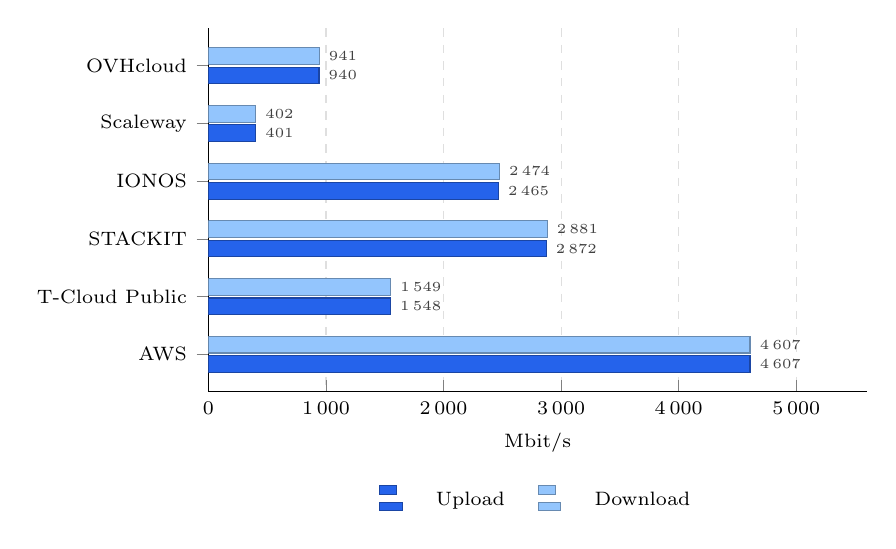
\begin{tikzpicture}
    \begin{axis}[benchh, xbar, /pgf/bar shift=0pt, height=6.2cm, xmin=0, xmax=5600,
      xlabel={Mbit/s}, /pgf/bar width=6pt,
      legend style={font=\scriptsize, at={(0.5,-0.24)}, anchor=north,
                    legend columns=2, draw=none, column sep=1em},
      nodes near coords={\pgfmathprintnumber[fixed, precision=0, 1000 sep={\,}]{\pgfplotspointmeta}},
      point meta=x]
      \addplot[fill=bSerA, draw=bSerA!70!black, /pgf/bar shift=-3.5pt] coordinates {(940.27,OVH) (400.99,SCW) (2465.30,ION) (2871.97,STK) (1548.00,TCL) (4607.00,AWS)};
      \addplot[fill=bSerB, draw=bSerB!70!black, /pgf/bar shift=3.5pt] coordinates {(941.20,OVH) (401.51,SCW) (2474.30,ION) (2880.97,STK) (1549.00,TCL) (4607.00,AWS)};
      \legend{Upload, Download}
    \end{axis}
  \end{tikzpicture}
  \caption{Network bandwidth between two machines in the same zone, \texttt{iperf3}.}
  \label{fig:bench-iperf}
\end{figure}

Network bandwidth separates the providers more than any other measurement.
\Cref{fig:bench-iperf} shows \acs{AWS} at 4\,607 Mbit/s, followed by STACKIT at 2\,872 and
IONOS at 2\,465; T-Cloud Public reaches 1\,548, OVHcloud 940, and Scaleway 401. The
bandwidth of \acs{AWS}, the fastest, is 11.5 times that of Scaleway, the slowest.
Upload and download are almost identical
for every provider.

Four of these results come from Cloud Mercato rather than from this study's own
measurements, and they were obtained differently. Cloud Mercato ran iperf3
between two machines in the same zone many times, varying the number of parallel
streams: 80 runs in each direction with one to four streams for \acs{AWS}, 50 with
one, two and four for T-Cloud Public, and 20 with two for Scaleway and StackIT
\cite{CloudMercato_AWS_m6i,CloudMercato_TSystems_s3,CloudMercato_Scaleway_POP2}.
The other two providers were measured in this study with three runs each. The
two sets are comparable in what they measure, but not in the number of runs
behind each figure.

The \acs{AWS} figure is the least stable of any in this study. The reported 80 runs range
from 758 to 11\,271 Mbit/s, and the spread does not follow the number of streams: with
one, two, three or four streams alike, results ran from about 760 to more than
9\,000 Mbit/s \cite{CloudMercato_AWS_m6i}. The average of 4\,607 Mbit/s therefore summarises a
result that varies by a factor of more than ten from one run to the next. The
Scaleway figure, by contrast, is stable and matches the product: Cloud Mercato
lists the network of this instance type at 381 Mbps, and the measured runs lie
between 390 and 462 \cite{CloudMercato_Scaleway_POP2}. The low figure for Scaleway
reflects the bandwidth the instance is sold with, not a fault in the
measurement.

\subsubsection{Provisioning time}

\begin{figure}[htbp]
  \centering
  \begin{tikzpicture}
    \begin{groupplot}[benchh,
      group style={group size=2 by 1, horizontal sep=0.6cm},
      width=0.5\textwidth, height=5.4cm, xmin=0,
      title style={font=\scriptsize\bfseries, yshift=-4pt},
      nodes near coords={\pgfmathprintnumber[fixed, precision=1, fixed zerofill]{\pgfplotspointmeta}}, point meta=x]
    \nextgroupplot[title={Boot time}, xmax=19, xlabel={seconds}]
      \addplot[fill=cProvB, draw=cProvB!70!black] coordinates {(10.63,OVH)};
      \addplot[fill=cProvA, draw=cProvA!70!black] coordinates {(14.10,SCW)};
      \addplot[fill=cProvD, draw=cProvD!70!black] coordinates {(15.27,ION)};
      \addplot[fill=cProvE, draw=cProvE!70!black] coordinates {(13.13,STK)};
      \addplot[fill=cProvC, draw=cProvC!70!black] coordinates {(15.80,TCL)};
      \addplot[fill=cBase, draw=cBase!70!black] coordinates {(13.30,AWS)};
    \nextgroupplot[title={Set-up time}, xmax=48, xlabel={seconds}, yticklabels={}]
      \addplot[fill=cProvB, draw=cProvB!70!black] coordinates {(22.27,OVH)};
      \addplot[fill=cProvA, draw=cProvA!70!black] coordinates {(34.43,SCW)};
      \addplot[fill=cProvD, draw=cProvD!70!black] coordinates {(28.80,ION)};
      \addplot[fill=cProvE, draw=cProvE!70!black] coordinates {(26.23,STK)};
      \addplot[fill=cProvC, draw=cProvC!70!black] coordinates {(39.80,TCL)};
      \addplot[fill=cBase, draw=cBase!70!black] coordinates {(23.40,AWS)};
    \end{groupplot}
  \end{tikzpicture}
  \caption{Time to boot until SSH is available, and to complete set-up, in seconds.}
  \label{fig:bench-bootsetup}
\end{figure}

\begin{figure}[htbp]
  \centering
  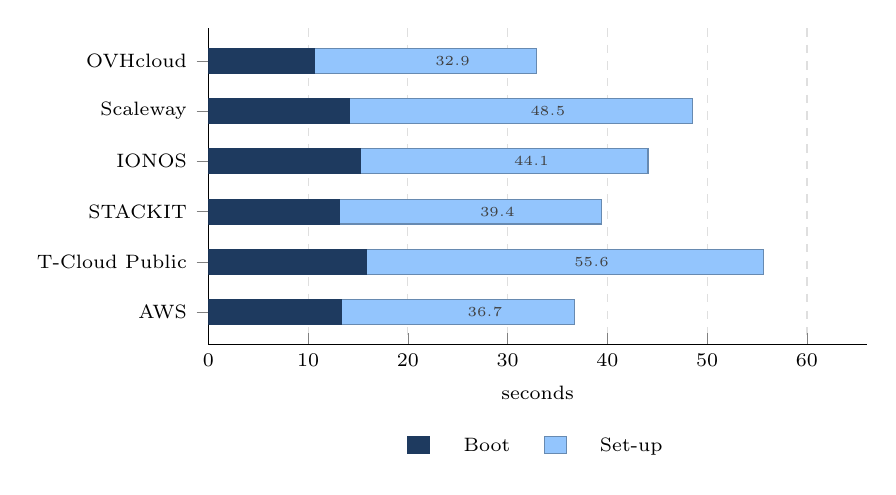
\begin{tikzpicture}
    \begin{axis}[benchh, xbar stacked, /pgf/bar shift=0pt, height=5.6cm, xmin=0, xmax=66,
      xlabel={seconds},
      legend style={font=\scriptsize, at={(0.5,-0.26)}, anchor=north,
                    legend columns=2, draw=none, column sep=1em}]
      \addplot[fill=bNavy, draw=bNavy] coordinates {(10.63,OVH) (14.10,SCW) (15.27,ION) (13.13,STK) (15.80,TCL) (13.30,AWS)};
      \addplot[fill=bSerB, draw=bSerB!70!black,
        nodes near coords={\pgfmathprintnumber[fixed, precision=1, fixed zerofill]{\pgfplotspointmeta}},
        point meta=explicit] coordinates {(22.27,OVH) [32.9] (34.43,SCW) [48.5] (28.80,ION) [44.1] (26.23,STK) [39.4] (39.80,TCL) [55.6] (23.40,AWS) [36.7]};
      \legend{Boot, Set-up}
    \end{axis}
  \end{tikzpicture}
  \caption{Total provisioning time, boot and set-up combined, in seconds.}
  \label{fig:bench-total}
\end{figure}

Every machine was ready for work in under a minute. OVHcloud boots fastest, in
10.63 seconds, and completes set-up fastest, in 22.27, so that it is ready in 32.9 seconds
in total (\cref{fig:bench-bootsetup,fig:bench-total}). \acs{AWS} follows at 36.7
seconds and STACKIT at 39.4. T-Cloud Public takes longest, at 55.6 seconds, most of
the difference arising in set-up rather than in boot. The scale of these times has
changed considerably since Gillam et al.\ took their measurements: they recorded
average boot times of around two minutes for \acs{AWS} machines
\cite{Gillam_FairBenchmarking_2013}, against between 10.63 and 15.8 seconds for every
provider here.

\subsection{Normalised comparison}
\label{sec:bench-composite}

Each test reports in its own unit, and the units cannot be added together. To
combine them, each result is expressed as a score out of 100 relative to the best
of the six providers on that test. For the six tests where a higher value is
better, the score is the provider's value divided by the best value; for boot and
set-up time, where a lower value is better, it is the best value divided by the
provider's. The composite score is the unweighted average of the eight:

\begin{equation}
  \label{eq:bench-score}
  s_{i} = 100 \times \frac{x_{i}}{\max_{j} x_{j}}
  \quad\text{or}\quad
  s_{i} = 100 \times \frac{\min_{j} x_{j}}{x_{i}},
  \qquad
  \text{composite} = \frac{1}{8}\sum_{m=1}^{8} s_{i,m}
\end{equation}

This follows Gillam et al.\ in setting each provider against the best result
achieved rather than against an external standard
\cite{Gillam_FairBenchmarking_2013}. \Cref{tab:bench-heatmap} gives every
measurement with its range, in the manner of their results tables, and colours
each cell by its score.

\begin{table}[htbp]
  \centering
  \caption{All eight measurements: the average, with the highest and lowest run
           beside it. Cell colour shows the score out of 100, and a box marks the
           best result in each column.}
  \label{tab:bench-heatmap}
  \scriptsize
  \setlength{\tabcolsep}{1.2pt}
  \renewcommand{\arraystretch}{1.5}
  \begin{tabular}{@{}>{\raggedright\arraybackslash}m{1.25cm} *{8}{>{\centering\arraybackslash}m{1.55cm}} >{\centering\arraybackslash}m{0.8cm}@{}}
    \toprule
    Provider & \shortstack{\textbf{Memory}\\[-1pt]{\tiny TRIAD}} & \shortstack{\textbf{CPU single}\\[-1pt]{\tiny hint}} & \shortstack{\textbf{CPU multi}\\[-1pt]{\tiny 7-zip}} & \shortstack{\textbf{Disk}\\[-1pt]{\tiny postmark}} & \shortstack{\textbf{Web}\\[-1pt]{\tiny apache}} & \shortstack{\textbf{Network}\\[-1pt]{\tiny iperf3}} & \shortstack{\textbf{Boot}\\[-1pt]{\tiny s, lower}} & \shortstack{\textbf{Set-up}\\[-1pt]{\tiny s, lower}} & \shortstack{\textbf{Comp.}\\[-1pt]{\tiny of 8}} \\
    \midrule
    AWS & \cellcolor[RGB]{187,247,208}\color[HTML]{14532D}{\setlength{\fboxsep}{1.2pt}\setlength{\fboxrule}{0.7pt}\color[RGB]{202,138,4}\fbox{\color[HTML]{14532D}\begin{tabular}{@{}r@{\hspace{2.5pt}}l@{}}{\fontsize{4.6}{5.3}\selectfont\color[HTML]{6D947D}\shortstack[r]{$\uparrow$21\,590\\$\downarrow$21\,351}} & \textbf{21\,477}\end{tabular}}} & \cellcolor[RGB]{187,247,208}\color[HTML]{14532D}\begin{tabular}{@{}r@{\hspace{2.5pt}}l@{}}{\fontsize{4.6}{5.3}\selectfont\color[HTML]{6D947D}\shortstack[r]{$\uparrow$445.9\\$\downarrow$441.3}} & 443.6\end{tabular} & \cellcolor[RGB]{206,248,196}\color[HTML]{14532D}\begin{tabular}{@{}r@{\hspace{2.5pt}}l@{}}{\fontsize{4.6}{5.3}\selectfont\color[HTML]{6D947D}\shortstack[r]{$\uparrow$10\,319\\$\downarrow$10\,275}} & 10\,296\end{tabular} & \cellcolor[RGB]{250,252,169}\color[HTML]{713F12}\begin{tabular}{@{}r@{\hspace{2.5pt}}l@{}}{\fontsize{4.6}{5.3}\selectfont\color[HTML]{A7886C}\shortstack[r]{$\uparrow$4\,510\\$\downarrow$4\,420}} & 4\,470\end{tabular} & \cellcolor[RGB]{196,248,202}\color[HTML]{14532D}\begin{tabular}{@{}r@{\hspace{2.5pt}}l@{}}{\fontsize{4.6}{5.3}\selectfont\color[HTML]{6D947D}\shortstack[r]{$\uparrow$30\,421\\$\downarrow$29\,850}} & 30\,127\end{tabular} & \cellcolor[RGB]{187,247,208}\color[HTML]{14532D}{\setlength{\fboxsep}{1.2pt}\setlength{\fboxrule}{0.7pt}\color[RGB]{202,138,4}\fbox{\color[HTML]{14532D}\begin{tabular}{@{}r@{\hspace{2.5pt}}l@{}}{\fontsize{4.6}{5.3}\selectfont\color[HTML]{6D947D}\shortstack[r]{$\uparrow$11\,271\\$\downarrow$758}} & \textbf{4\,607}\end{tabular}}} & \cellcolor[RGB]{214,249,191}\color[HTML]{14532D}\begin{tabular}{@{}r@{\hspace{2.5pt}}l@{}}{\fontsize{4.6}{5.3}\selectfont\color[HTML]{6D947D}\shortstack[r]{$\uparrow$13.8\\$\downarrow$12.9}} & 13.3\end{tabular} & \cellcolor[RGB]{194,248,204}\color[HTML]{14532D}\begin{tabular}{@{}r@{\hspace{2.5pt}}l@{}}{\fontsize{4.6}{5.3}\selectfont\color[HTML]{6D947D}\shortstack[r]{$\uparrow$24.8\\$\downarrow$22.1}} & 23.4\end{tabular} & \cellcolor[RGB]{203,248,198}\color[HTML]{14532D}\textbf{88.4} \\
    OVHcloud & \cellcolor[RGB]{215,249,190}\color[HTML]{14532D}\begin{tabular}{@{}r@{\hspace{2.5pt}}l@{}}{\fontsize{4.6}{5.3}\selectfont\color[HTML]{6D947D}\shortstack[r]{$\uparrow$16\,988\\$\downarrow$16\,900}} & 16\,944\end{tabular} & \cellcolor[RGB]{187,247,208}\color[HTML]{14532D}{\setlength{\fboxsep}{1.2pt}\setlength{\fboxrule}{0.7pt}\color[RGB]{202,138,4}\fbox{\color[HTML]{14532D}\begin{tabular}{@{}r@{\hspace{2.5pt}}l@{}}{\fontsize{4.6}{5.3}\selectfont\color[HTML]{6D947D}\shortstack[r]{$\uparrow$448.5\\$\downarrow$442.1}} & \textbf{445.3}\end{tabular}}} & \cellcolor[RGB]{187,247,208}\color[HTML]{14532D}{\setlength{\fboxsep}{1.2pt}\setlength{\fboxrule}{0.7pt}\color[RGB]{202,138,4}\fbox{\color[HTML]{14532D}\begin{tabular}{@{}r@{\hspace{2.5pt}}l@{}}{\fontsize{4.6}{5.3}\selectfont\color[HTML]{6D947D}\shortstack[r]{$\uparrow$12\,100\\$\downarrow$11\,850}} & \textbf{11\,977}\end{tabular}}} & \cellcolor[RGB]{187,247,208}\color[HTML]{14532D}{\setlength{\fboxsep}{1.2pt}\setlength{\fboxrule}{0.7pt}\color[RGB]{202,138,4}\fbox{\color[HTML]{14532D}\begin{tabular}{@{}r@{\hspace{2.5pt}}l@{}}{\fontsize{4.6}{5.3}\selectfont\color[HTML]{6D947D}\shortstack[r]{$\uparrow$8\,480\\$\downarrow$8\,250}} & \textbf{8\,363}\end{tabular}}} & \cellcolor[RGB]{187,247,208}\color[HTML]{14532D}{\setlength{\fboxsep}{1.2pt}\setlength{\fboxrule}{0.7pt}\color[RGB]{202,138,4}\fbox{\color[HTML]{14532D}\begin{tabular}{@{}r@{\hspace{2.5pt}}l@{}}{\fontsize{4.6}{5.3}\selectfont\color[HTML]{6D947D}\shortstack[r]{$\uparrow$32\,850\\$\downarrow$32\,101}} & \textbf{32\,477}\end{tabular}}} & \cellcolor[RGB]{254,222,188}\color[HTML]{7F1D1D}\begin{tabular}{@{}r@{\hspace{2.5pt}}l@{}}{\fontsize{4.6}{5.3}\selectfont\color[HTML]{B07373}\shortstack[r]{$\uparrow$943\\$\downarrow$938}} & 940\end{tabular} & \cellcolor[RGB]{187,247,208}\color[HTML]{14532D}{\setlength{\fboxsep}{1.2pt}\setlength{\fboxrule}{0.7pt}\color[RGB]{202,138,4}\fbox{\color[HTML]{14532D}\begin{tabular}{@{}r@{\hspace{2.5pt}}l@{}}{\fontsize{4.6}{5.3}\selectfont\color[HTML]{6D947D}\shortstack[r]{$\uparrow$11.1\\$\downarrow$10.2}} & \textbf{10.63}\end{tabular}}} & \cellcolor[RGB]{187,247,208}\color[HTML]{14532D}{\setlength{\fboxsep}{1.2pt}\setlength{\fboxrule}{0.7pt}\color[RGB]{202,138,4}\fbox{\color[HTML]{14532D}\begin{tabular}{@{}r@{\hspace{2.5pt}}l@{}}{\fontsize{4.6}{5.3}\selectfont\color[HTML]{6D947D}\shortstack[r]{$\uparrow$23.2\\$\downarrow$21.5}} & \textbf{22.27}\end{tabular}}} & \cellcolor[RGB]{204,248,197}\color[HTML]{14532D}\textbf{87.4} \\
    STACKIT & \cellcolor[RGB]{203,248,198}\color[HTML]{14532D}\begin{tabular}{@{}r@{\hspace{2.5pt}}l@{}}{\fontsize{4.6}{5.3}\selectfont\color[HTML]{6D947D}\shortstack[r]{$\uparrow$19\,110\\$\downarrow$18\,851}} & 18\,994\end{tabular} & \cellcolor[RGB]{194,248,204}\color[HTML]{14532D}\begin{tabular}{@{}r@{\hspace{2.5pt}}l@{}}{\fontsize{4.6}{5.3}\selectfont\color[HTML]{6D947D}\shortstack[r]{$\uparrow$426.8\\$\downarrow$421.4}} & 424.3\end{tabular} & \cellcolor[RGB]{203,248,198}\color[HTML]{14532D}\begin{tabular}{@{}r@{\hspace{2.5pt}}l@{}}{\fontsize{4.6}{5.3}\selectfont\color[HTML]{6D947D}\shortstack[r]{$\uparrow$10\,550\\$\downarrow$10\,420}} & 10\,483\end{tabular} & \cellcolor[RGB]{222,250,186}\color[HTML]{713F12}\begin{tabular}{@{}r@{\hspace{2.5pt}}l@{}}{\fontsize{4.6}{5.3}\selectfont\color[HTML]{A7886C}\shortstack[r]{$\uparrow$6\,280\\$\downarrow$6\,120}} & 6\,203\end{tabular} & \cellcolor[RGB]{202,248,199}\color[HTML]{14532D}\begin{tabular}{@{}r@{\hspace{2.5pt}}l@{}}{\fontsize{4.6}{5.3}\selectfont\color[HTML]{6D947D}\shortstack[r]{$\uparrow$29\,100\\$\downarrow$28\,451}} & 28\,790\end{tabular} & \cellcolor[RGB]{238,251,176}\color[HTML]{713F12}\begin{tabular}{@{}r@{\hspace{2.5pt}}l@{}}{\fontsize{4.6}{5.3}\selectfont\color[HTML]{A7886C}\shortstack[r]{$\uparrow$2\,891\\$\downarrow$2\,850}} & 2\,872\end{tabular} & \cellcolor[RGB]{212,249,192}\color[HTML]{14532D}\begin{tabular}{@{}r@{\hspace{2.5pt}}l@{}}{\fontsize{4.6}{5.3}\selectfont\color[HTML]{6D947D}\shortstack[r]{$\uparrow$13.5\\$\downarrow$12.8}} & 13.13\end{tabular} & \cellcolor[RGB]{207,249,195}\color[HTML]{14532D}\begin{tabular}{@{}r@{\hspace{2.5pt}}l@{}}{\fontsize{4.6}{5.3}\selectfont\color[HTML]{6D947D}\shortstack[r]{$\uparrow$27.1\\$\downarrow$25.4}} & 26.23\end{tabular} & \cellcolor[RGB]{210,249,194}\color[HTML]{14532D}\textbf{82.8} \\
    IONOS & \cellcolor[RGB]{194,248,204}\color[HTML]{14532D}\begin{tabular}{@{}r@{\hspace{2.5pt}}l@{}}{\fontsize{4.6}{5.3}\selectfont\color[HTML]{6D947D}\shortstack[r]{$\uparrow$20\,510\\$\downarrow$20\,251}} & 20\,394\end{tabular} & \cellcolor[RGB]{196,248,202}\color[HTML]{14532D}\begin{tabular}{@{}r@{\hspace{2.5pt}}l@{}}{\fontsize{4.6}{5.3}\selectfont\color[HTML]{6D947D}\shortstack[r]{$\uparrow$418.9\\$\downarrow$412.4}} & 415.6\end{tabular} & \cellcolor[RGB]{215,249,190}\color[HTML]{14532D}\begin{tabular}{@{}r@{\hspace{2.5pt}}l@{}}{\fontsize{4.6}{5.3}\selectfont\color[HTML]{6D947D}\shortstack[r]{$\uparrow$9\,510\\$\downarrow$9\,420}} & 9\,470\end{tabular} & \cellcolor[RGB]{227,250,183}\color[HTML]{713F12}\begin{tabular}{@{}r@{\hspace{2.5pt}}l@{}}{\fontsize{4.6}{5.3}\selectfont\color[HTML]{A7886C}\shortstack[r]{$\uparrow$5\,950\\$\downarrow$5\,820}} & 5\,893\end{tabular} & \cellcolor[RGB]{206,248,196}\color[HTML]{14532D}\begin{tabular}{@{}r@{\hspace{2.5pt}}l@{}}{\fontsize{4.6}{5.3}\selectfont\color[HTML]{6D947D}\shortstack[r]{$\uparrow$28\,100\\$\downarrow$27\,451}} & 27\,790\end{tabular} & \cellcolor[RGB]{249,252,169}\color[HTML]{713F12}\begin{tabular}{@{}r@{\hspace{2.5pt}}l@{}}{\fontsize{4.6}{5.3}\selectfont\color[HTML]{A7886C}\shortstack[r]{$\uparrow$2\,481\\$\downarrow$2\,450}} & 2\,465\end{tabular} & \cellcolor[RGB]{227,250,183}\color[HTML]{713F12}\begin{tabular}{@{}r@{\hspace{2.5pt}}l@{}}{\fontsize{4.6}{5.3}\selectfont\color[HTML]{A7886C}\shortstack[r]{$\uparrow$15.8\\$\downarrow$14.9}} & 15.27\end{tabular} & \cellcolor[RGB]{218,249,189}\color[HTML]{14532D}\begin{tabular}{@{}r@{\hspace{2.5pt}}l@{}}{\fontsize{4.6}{5.3}\selectfont\color[HTML]{6D947D}\shortstack[r]{$\uparrow$30.1\\$\downarrow$27.9}} & 28.8\end{tabular} & \cellcolor[RGB]{216,249,190}\color[HTML]{14532D}\textbf{78.0} \\
    \shortstack[l]{T-Cloud\\Public} & \cellcolor[RGB]{195,248,203}\color[HTML]{14532D}\begin{tabular}{@{}r@{\hspace{2.5pt}}l@{}}{\fontsize{4.6}{5.3}\selectfont\color[HTML]{6D947D}\shortstack[r]{$\uparrow$20\,250\\$\downarrow$19\,951}} & 20\,100\end{tabular} & \cellcolor[RGB]{195,248,203}\color[HTML]{14532D}\begin{tabular}{@{}r@{\hspace{2.5pt}}l@{}}{\fontsize{4.6}{5.3}\selectfont\color[HTML]{6D947D}\shortstack[r]{$\uparrow$421.8\\$\downarrow$415.2}} & 418.5\end{tabular} & \cellcolor[RGB]{194,248,204}\color[HTML]{14532D}\begin{tabular}{@{}r@{\hspace{2.5pt}}l@{}}{\fontsize{4.6}{5.3}\selectfont\color[HTML]{6D947D}\shortstack[r]{$\uparrow$11\,480\\$\downarrow$11\,250}} & 11\,363\end{tabular} & \cellcolor[RGB]{225,250,184}\color[HTML]{713F12}\begin{tabular}{@{}r@{\hspace{2.5pt}}l@{}}{\fontsize{4.6}{5.3}\selectfont\color[HTML]{A7886C}\shortstack[r]{$\uparrow$6\,150\\$\downarrow$5\,980}} & 6\,063\end{tabular} & \cellcolor[RGB]{192,247,205}\color[HTML]{14532D}\begin{tabular}{@{}r@{\hspace{2.5pt}}l@{}}{\fontsize{4.6}{5.3}\selectfont\color[HTML]{6D947D}\shortstack[r]{$\uparrow$31\,521\\$\downarrow$30\,850}} & 31\,184\end{tabular} & \cellcolor[RGB]{254,236,178}\color[HTML]{7F1D1D}\begin{tabular}{@{}r@{\hspace{2.5pt}}l@{}}{\fontsize{4.6}{5.3}\selectfont\color[HTML]{B07373}\shortstack[r]{$\uparrow$1\,578\\$\downarrow$1\,538}} & 1\,548\end{tabular} & \cellcolor[RGB]{231,250,180}\color[HTML]{713F12}\begin{tabular}{@{}r@{\hspace{2.5pt}}l@{}}{\fontsize{4.6}{5.3}\selectfont\color[HTML]{A7886C}\shortstack[r]{$\uparrow$16.4\\$\downarrow$15.2}} & 15.8\end{tabular} & \cellcolor[RGB]{246,251,171}\color[HTML]{713F12}\begin{tabular}{@{}r@{\hspace{2.5pt}}l@{}}{\fontsize{4.6}{5.3}\selectfont\color[HTML]{A7886C}\shortstack[r]{$\uparrow$41.2\\$\downarrow$38.5}} & 39.8\end{tabular} & \cellcolor[RGB]{219,249,188}\color[HTML]{14532D}\textbf{76.0} \\
    Scaleway & \cellcolor[RGB]{200,248,200}\color[HTML]{14532D}\begin{tabular}{@{}r@{\hspace{2.5pt}}l@{}}{\fontsize{4.6}{5.3}\selectfont\color[HTML]{6D947D}\shortstack[r]{$\uparrow$19\,490\\$\downarrow$19\,281}} & 19\,384\end{tabular} & \cellcolor[RGB]{190,247,206}\color[HTML]{14532D}\begin{tabular}{@{}r@{\hspace{2.5pt}}l@{}}{\fontsize{4.6}{5.3}\selectfont\color[HTML]{6D947D}\shortstack[r]{$\uparrow$439.9\\$\downarrow$435.1}} & 437.5\end{tabular} & \cellcolor[RGB]{199,248,200}\color[HTML]{14532D}\begin{tabular}{@{}r@{\hspace{2.5pt}}l@{}}{\fontsize{4.6}{5.3}\selectfont\color[HTML]{6D947D}\shortstack[r]{$\uparrow$10\,980\\$\downarrow$10\,850}} & 10\,917\end{tabular} & \cellcolor[RGB]{216,249,190}\color[HTML]{14532D}\begin{tabular}{@{}r@{\hspace{2.5pt}}l@{}}{\fontsize{4.6}{5.3}\selectfont\color[HTML]{6D947D}\shortstack[r]{$\uparrow$6\,580\\$\downarrow$6\,450}} & 6\,513\end{tabular} & \cellcolor[RGB]{199,248,200}\color[HTML]{14532D}\begin{tabular}{@{}r@{\hspace{2.5pt}}l@{}}{\fontsize{4.6}{5.3}\selectfont\color[HTML]{6D947D}\shortstack[r]{$\uparrow$29\,751\\$\downarrow$29\,100}} & 29\,424\end{tabular} & \cellcolor[RGB]{254,211,196}\color[HTML]{7F1D1D}\begin{tabular}{@{}r@{\hspace{2.5pt}}l@{}}{\fontsize{4.6}{5.3}\selectfont\color[HTML]{B07373}\shortstack[r]{$\uparrow$462\\$\downarrow$390}} & 401\end{tabular} & \cellcolor[RGB]{221,250,187}\color[HTML]{14532D}\begin{tabular}{@{}r@{\hspace{2.5pt}}l@{}}{\fontsize{4.6}{5.3}\selectfont\color[HTML]{6D947D}\shortstack[r]{$\uparrow$14.5\\$\downarrow$13.8}} & 14.1\end{tabular} & \cellcolor[RGB]{234,250,179}\color[HTML]{713F12}\begin{tabular}{@{}r@{\hspace{2.5pt}}l@{}}{\fontsize{4.6}{5.3}\selectfont\color[HTML]{A7886C}\shortstack[r]{$\uparrow$36.1\\$\downarrow$33.2}} & 34.43\end{tabular} & \cellcolor[RGB]{221,250,187}\color[HTML]{713F12}\textbf{74.6} \\
    \bottomrule
  \end{tabular}

  \vspace{4pt}
  {\scriptsize\raggedright Low \tikz\fill[fill={rgb,255:red,254;green,202;blue,202}] (0,0) rectangle (0.42,0.24); \tikz\fill[fill={rgb,255:red,254;green,222;blue,188}] (0,0) rectangle (0.42,0.24); \tikz\fill[fill={rgb,255:red,254;green,242;blue,173}] (0,0) rectangle (0.42,0.24); \tikz\fill[fill={rgb,255:red,241;green,251;blue,174}] (0,0) rectangle (0.42,0.24); \tikz\fill[fill={rgb,255:red,214;green,249;blue,191}] (0,0) rectangle (0.42,0.24); \tikz\fill[fill={rgb,255:red,187;green,247;blue,208}] (0,0) rectangle (0.42,0.24); High \quad Memory in MB/s, CPU single in million
  MIPS, CPU multi in MIPS, disk in transactions and web in requests per second,
  network in Mbit/s. Every value is the average of three runs, except network bandwidth for AWS (80), T-Cloud Public (50), Scaleway (20), which are Cloud Mercato's.\par}
\end{table}

\begin{figure}[htbp]
  \centering
  \begin{tikzpicture}
    \begin{axis}[benchh, xmin=0, xmax=105, xlabel={score out of 100},nodes near coords={\pgfmathprintnumber[fixed, precision=1, fixed zerofill]{\pgfplotspointmeta}},point meta=x]
      \addplot[fill=cProvB, draw=cProvB!70!black] coordinates {(87.4,OVH)};
      \addplot[fill=cProvA, draw=cProvA!70!black] coordinates {(74.6,SCW)};
      \addplot[fill=cProvD, draw=cProvD!70!black] coordinates {(78.0,ION)};
      \addplot[fill=cProvE, draw=cProvE!70!black] coordinates {(82.8,STK)};
      \addplot[fill=cProvC, draw=cProvC!70!black] coordinates {(76.0,TCL)};
      \addplot[fill=cBase, draw=cBase!70!black] coordinates {(88.4,AWS)};
    \end{axis}
  \end{tikzpicture}
  \caption{Composite performance score, the average of the eight normalised measurements.}
  \label{fig:bench-composite}
\end{figure}

The composite scores lie within 13.8 points of each other (\cref{fig:bench-composite}).
\acs{AWS} ranks first at 88.4, followed closely by OVHcloud at 87.4, then STACKIT
at 82.8, IONOS at 78.0, T-Cloud Public at 76.0 and Scaleway at 74.6. The ranking
at the top rests on a single measurement. OVHcloud records the best result on
six of the eight tests --- single-core and multi-core processing, disk, web
serving, boot and set-up --- and \acs{AWS} on the other two, memory and network.
On network bandwidth \acs{AWS} scores 100 while no European provider scores more
than 62, and that one column accounts for its lead: without it, OVHcloud's average
across the remaining seven tests would be 97.0 and that of \acs{AWS} 86.7.


\subsection{Price and value for money}

\begin{figure}[htbp]
  \centering
  \begin{tikzpicture}
    \begin{axis}[benchh, xmin=0, xmax=0.135, xlabel={euros per hour},nodes near coords={\texteuro\pgfmathprintnumber[fixed, precision=3, fixed zerofill]{\pgfplotspointmeta}},point meta=x, xtick={0,0.03,0.06,0.09,0.12}, xticklabel style={/pgf/number format/fixed, /pgf/number format/precision=2}]
      \addplot[fill=cProvB, draw=cProvB!70!black] coordinates {(0.060,OVH)};
      \addplot[fill=cProvA, draw=cProvA!70!black] coordinates {(0.074,SCW)};
      \addplot[fill=cProvD, draw=cProvD!70!black] coordinates {(0.041,ION)};
      \addplot[fill=cProvE, draw=cProvE!70!black] coordinates {(0.098,STK)};
      \addplot[fill=cProvC, draw=cProvC!70!black] coordinates {(0.114,TCL)};
      \addplot[fill=cBase, draw=cBase!70!black] coordinates {(0.106,AWS)};
    \end{axis}
  \end{tikzpicture}
  \caption{Hourly list price, 2\,vCPU and 8\,GB of memory.}
  \label{fig:bench-price}
\end{figure}

\begin{figure}[htbp]
  \centering
  \begin{tikzpicture}
    \begin{axis}[benchh, height=5.4cm, xmin=0, xmax=2250, xlabel={composite score per euro per hour},
      symbolic y coords={V0,V1,V2,V3,V4,V5}, ytick={V0,V1,V2,V3,V4,V5},
      yticklabels={IONOS,OVHcloud,Scaleway,STACKIT,AWS,{T-Cloud Public}},
      nodes near coords={\pgfmathprintnumber[fixed, precision=0, 1000 sep={\,}]{\pgfplotspointmeta}},
      point meta=x]
      \addplot[fill=cProvD, draw=cProvD!70!black] coordinates {(1902,V0)};
      \addplot[fill=cProvB, draw=cProvB!70!black] coordinates {(1457,V1)};
      \addplot[fill=cProvA, draw=cProvA!70!black] coordinates {(1008,V2)};
      \addplot[fill=cProvE, draw=cProvE!70!black] coordinates {(845,V3)};
      \addplot[fill=cBase, draw=cBase!70!black] coordinates {(834,V4)};
      \addplot[fill=cProvC, draw=cProvC!70!black] coordinates {(667,V5)};
    \end{axis}
  \end{tikzpicture}
  \caption{Composite score per euro per hour, ordered from the best value.}
  \label{fig:bench-value}
\end{figure}

\begin{figure}[htbp]
  \centering
  \begin{tikzpicture}
    \begin{groupplot}[benchh,
      group style={group size=2 by 3, horizontal sep=0.6cm, vertical sep=1.2cm},
      width=0.5\textwidth, height=4.6cm, xmin=0, xmax=2800,
      xtick={0,1000,2000}, xticklabels={0,1k,2k}, /pgf/bar width=6pt,
      title style={font=\scriptsize\bfseries, yshift=-4pt},
      nodes near coords={\pgfmathprintnumber[fixed, precision=0, 1000 sep={\,}]{\pgfplotspointmeta}},
      nodes near coords style={font=\tiny, anchor=west, black!75},
      point meta=x]
    \nextgroupplot[title={Memory / \texteuro}]
      \addplot[fill=cProvB, draw=cProvB!70!black] coordinates {(1317,OVH)};
      \addplot[fill=cProvA, draw=cProvA!70!black] coordinates {(1216,SCW)};
      \addplot[fill=cProvD, draw=cProvD!70!black] coordinates {(2317,ION)};
      \addplot[fill=cProvE, draw=cProvE!70!black] coordinates {(898,STK)};
      \addplot[fill=cProvC, draw=cProvC!70!black] coordinates {(825,TCL)};
      \addplot[fill=cBase, draw=cBase!70!black] coordinates {(943,AWS)};
    \nextgroupplot[title={CPU single / \texteuro}, yticklabels={}]
      \addplot[fill=cProvB, draw=cProvB!70!black] coordinates {(1667,OVH)};
      \addplot[fill=cProvA, draw=cProvA!70!black] coordinates {(1324,SCW)};
      \addplot[fill=cProvD, draw=cProvD!70!black] coordinates {(2268,ION)};
      \addplot[fill=cProvE, draw=cProvE!70!black] coordinates {(969,STK)};
      \addplot[fill=cProvC, draw=cProvC!70!black] coordinates {(825,TCL)};
      \addplot[fill=cBase, draw=cBase!70!black] coordinates {(943,AWS)};
    \nextgroupplot[title={CPU multi / \texteuro}]
      \addplot[fill=cProvB, draw=cProvB!70!black] coordinates {(1667,OVH)};
      \addplot[fill=cProvA, draw=cProvA!70!black] coordinates {(1230,SCW)};
      \addplot[fill=cProvD, draw=cProvD!70!black] coordinates {(1927,ION)};
      \addplot[fill=cProvE, draw=cProvE!70!black] coordinates {(898,STK)};
      \addplot[fill=cProvC, draw=cProvC!70!black] coordinates {(833,TCL)};
      \addplot[fill=cBase, draw=cBase!70!black] coordinates {(811,AWS)};
    \nextgroupplot[title={Disk / \texteuro}, yticklabels={}]
      \addplot[fill=cProvB, draw=cProvB!70!black] coordinates {(1667,OVH)};
      \addplot[fill=cProvA, draw=cProvA!70!black] coordinates {(1054,SCW)};
      \addplot[fill=cProvD, draw=cProvD!70!black] coordinates {(1707,ION)};
      \addplot[fill=cProvE, draw=cProvE!70!black] coordinates {(755,STK)};
      \addplot[fill=cProvC, draw=cProvC!70!black] coordinates {(632,TCL)};
      \addplot[fill=cBase, draw=cBase!70!black] coordinates {(500,AWS)};
    \nextgroupplot[title={Web / \texteuro}]
      \addplot[fill=cProvB, draw=cProvB!70!black] coordinates {(1667,OVH)};
      \addplot[fill=cProvA, draw=cProvA!70!black] coordinates {(1230,SCW)};
      \addplot[fill=cProvD, draw=cProvD!70!black] coordinates {(2098,ION)};
      \addplot[fill=cProvE, draw=cProvE!70!black] coordinates {(908,STK)};
      \addplot[fill=cProvC, draw=cProvC!70!black] coordinates {(842,TCL)};
      \addplot[fill=cBase, draw=cBase!70!black] coordinates {(877,AWS)};
    \nextgroupplot[title={Network / \texteuro}, yticklabels={}]
      \addplot[fill=cProvB, draw=cProvB!70!black] coordinates {(333,OVH)};
      \addplot[fill=cProvA, draw=cProvA!70!black] coordinates {(122,SCW)};
      \addplot[fill=cProvD, draw=cProvD!70!black] coordinates {(1317,ION)};
      \addplot[fill=cProvE, draw=cProvE!70!black] coordinates {(633,STK)};
      \addplot[fill=cProvC, draw=cProvC!70!black] coordinates {(298,TCL)};
      \addplot[fill=cBase, draw=cBase!70!black] coordinates {(943,AWS)};
    \end{groupplot}
  \end{tikzpicture}
  \caption{Score per euro per hour for each measurement.}
  \label{fig:bench-value-metric}
\end{figure}

The hourly list prices recorded at the time of testing range from \texteuro0.041 for IONOS
to \texteuro0.114 for T-Cloud Public (\cref{fig:bench-price}). \acs{AWS}, at \texteuro0.106, is the second
most expensive of the six. Dividing the composite score by the hourly price gives
the performance obtained for each euro, shown in \cref{fig:bench-value}. On this
measure the order changes almost completely. IONOS delivers the most performance
per euro, 2.3 times as much as \acs{AWS}, because it has the lowest price and a
composite only 10.4 points below the leader; OVHcloud is second at 1.7 times
\acs{AWS}. T-Cloud Public, with the highest price, delivers the least.
\Cref{fig:bench-value-metric} shows the same calculation for each measurement
separately: IONOS delivers the most per euro on every one of the six, including
network bandwidth, the one measurement on which \acs{AWS} leads outright.


\subsection{Findings and scope}
\label{sec:bench-findings}

On a machine of the same size, the European providers are not behind the
baseline. OVHcloud matches or exceeds \acs{AWS} on six of the eight measurements at
57 per cent of its hourly price, and four European providers --- OVHcloud,
T-Cloud Public, Scaleway and STACKIT --- outperform it when all processor cores
are in use.
The capability gap measured in \cref{sec:method-study2} and the financial gap
measured in \cref{sec:method-study3} concern the breadth of what a provider
offers and the resources behind it; neither reappears in the performance of an
individual machine. The one clear advantage of \acs{AWS} is network bandwidth
between machines, which matters most to applications spread across many of them.
Measured per euro, IONOS and OVHcloud offer the most performance of the six, and
the highest-priced provider, T-Cloud Public, the least.

These results describe one size of machine, in one region per provider, measured
on a single day. Measured against the principles of Papadopoulos et al., the study
describes its set-up, states its units, reports each result with its range and
includes cost, but it falls short on two of them
\cite{Papadopoulos_Principles_2021}. Each of the author's measurements rests on
three runs, whereas Gillam et al.\ typically ran ten for each machine type and
found that machines of the same specification from the same provider can differ
substantially in performance \cite{Gillam_FairBenchmarking_2013}; and with three
runs, no statistical test of the differences between providers was possible. The
research reviewed above also shows that variation differs between providers and
that providers change their infrastructure over time
\cite{LeitnerCito_Chaos_2016}. The comparison therefore establishes that European
performance is competitive at this size and price on the date it was measured; it
does not establish how consistently a newly provisioned machine will deliver it,
or whether the ranking will hold as the providers renew their hardware.
